\newcommand{\svcourse}{CST Part IA: Software Engineering and Security}
\newcommand{\svnumber}{1}
\newcommand{\svvenue}{Microsoft Teams}
\newcommand{\svdate}{2022-05-11}
\newcommand{\svtime}{15:00}
\newcommand{\svuploadkey}{CBd13xmL7PC1zqhNIoLdTiYUBnxZhzRAtJxv/ytRdM1r7qIfwMsxeVwM/pPcIo8l}

\newcommand{\svrname}{Dr Sam Ainsworth}
\newcommand{\jkfside}{oneside}
\newcommand{\jkfhanded}{yes}

\newcommand{\studentname}{Harry Langford}
\newcommand{\studentemail}{hjel2@cam.ac.uk}


\documentclass[10pt,\jkfside,a4paper]{article}
\usepackage{graphicx}
\usepackage{float}
\usepackage{color}

% DO NOT add \usepackage commands here.  Place any custom commands
% into your SV work files.  Anything in the template directory is
% likely to be overwritten!

\usepackage{fancyhdr}

\usepackage{lastpage}       % ``n of m'' page numbering
\usepackage{lscape}         % Makes landscape easier

\usepackage{verbatim}       % Verbatim blocks
\usepackage{listings}       % Source code listings
\usepackage{graphicx}
\usepackage{float}
\usepackage{epsfig}         % Embed encapsulated postscript
\usepackage{array}          % Array environment
\usepackage{qrcode}         % QR codes
\usepackage{enumitem}       % Required by Tom Johnson's exam question header

\usepackage{hhline}         % Horizontal lines in tables
\usepackage{siunitx}        % Correct spacing of units
\usepackage{amsmath}        % American Mathematical Society
\usepackage{amssymb}        % Maths symbols
\usepackage{amsthm}         % Theorems

\usepackage{ifthen}         % Conditional processing in tex

\usepackage[top=3cm,
            bottom=3cm,
            inner=2cm,
            outer=5cm]{geometry}

% PDF metadata + URL formatting
\usepackage[
            pdfauthor={\studentname},
            pdftitle={\svcourse, SV \svnumber},
            pdfsubject={},
            pdfkeywords={9d2547b00aba40b58fa0378774f72ee6},
            pdfproducer={},
            pdfcreator={},
            hidelinks]{hyperref}

\renewcommand{\headrulewidth}{0.4pt}
\renewcommand{\footrulewidth}{0.4pt}
\fancyheadoffset[LO,LE,RO,RE]{0pt}
\fancyfootoffset[LO,LE,RO,RE]{0pt}
\pagestyle{fancy}
\fancyhead{}
\fancyhead[LO,RE]{{\bfseries \studentname}\\\studentemail}
\fancyhead[RO,LE]{{\bfseries \svcourse, SV~\svnumber}\\\svdate\ \svtime, \svvenue}
\fancyfoot{}
\fancyfoot[LO,RE]{For: \svrname}
\fancyfoot[RO,LE]{\today\hspace{1cm}\thepage\ / \pageref{LastPage}}
\fancyfoot[C]{\qrcode[height=0.8cm]{\svuploadkey}}
\setlength{\headheight}{22.55pt}


\ifthenelse{\equal{\jkfside}{oneside}}{

 \ifthenelse{\equal{\jkfhanded}{left}}{
  % 1. Left-handed marker, one-sided printing or e-marking, use oneside and...
  \evensidemargin=\oddsidemargin
  \oddsidemargin=73pt
  \setlength{\marginparwidth}{111pt}
  \setlength{\marginparsep}{-\marginparsep}
  \addtolength{\marginparsep}{-\textwidth}
  \addtolength{\marginparsep}{-\marginparwidth}
 }{
  % 2. Right-handed marker, one-sided printing or e-marking, use oneside.
  \setlength{\marginparwidth}{111pt}
 }

}{
 % 3. Alternating margins, two-sided printing, use twoside.
}


\setlength{\parindent}{0em}
\addtolength{\parskip}{1ex}

% Exam question headings, labels and sensible layout (courtesy of Tom Johnson)
\setlist{parsep=\parskip, listparindent=\parindent}
\newcommand{\examhead}[3]{\section{#1 Paper #2 Question #3}}
\newenvironment{examquestion}[3]{
\examhead{#1}{#2}{#3}\setlist[enumerate, 1]{label=(\alph*)}\setlist[enumerate, 2]{label=(\roman*)}
\marginpar{\href{https://www.cl.cam.ac.uk/teaching/exams/pastpapers/y#1p#2q#3.pdf}{\qrcode{https://www.cl.cam.ac.uk/teaching/exams/pastpapers/y#1p#2q#3.pdf}}}
\marginpar{\footnotesize \href{https://www.cl.cam.ac.uk/teaching/exams/pastpapers/y#1p#2q#3.pdf}{https://www.cl.cam.ac.uk/\\teaching/exams/pastpapers/\\y#1p#2q#3.pdf}}
}{}


\begin{document}

\section{Further Graphics Exercise Set II}

\begin{enumerate}

\item Simple 3D engines often approximate lighting as the
superposition/combination of diffuse ambient light and direct illumination
from point sources. This is a rather crude (yet efficient) approximation to
the full rendering equation. What kind of effects are not captured by this
simple approximation, i.e. what kind of visual effects cannot be rendered.

\begin{itemize}

\item Reflections

\item Caustics

\item Soft shadows

\end{itemize}

{\color{blue}
You can't have transparent objects.

The crude approximation for transparent objects is alpha blending. You
render the object behind and then render the first surface with $\alpha$.

Fog

Indirect illumination -- requiring illumination from other objects which are
nearby ie ambient occlusion
}

\item If there is only diffuse ambient light, we can easily determine the
radiosity of a point on the surface through ambient occlusion, i.e.\ by
measuring how much of the ``sky'' is visible from that specific point.

Briefly describe how information about the curvature of a surface can help
in this situation.

In this situation, linear interpolation can provide a good approximation to
the surface. However, linearly interpolating over a curved surface will give
artefacts. Knowing the curvature of the surface informs us of how much we
can interpolate and when we should resample.

{
\color{blue}
Under this, we can approximate the light by curvature. If a surface has a
high positive curvature (in a deep trench) then the light is very low.
If a surface has a zero or negative curvature then we can give it the normal
light.

IE approximate ambient occlusion can be approximated by curvature.

Ambient occlusion picks up high-frequency features which would otherwise be
saturated.
}

\item Consider the function $f(x)$ with the graph shown below. In the range
0 to 10, it covers an area of
$I = \int^{10}_0 f(x)\text{d}x \approx 4.329268516$.

\[
f(x) = \frac{40}{(1 + e^x)\cdot ((x - 2)^4 + 4)}
\]

\begin{figure}[H]
\centering
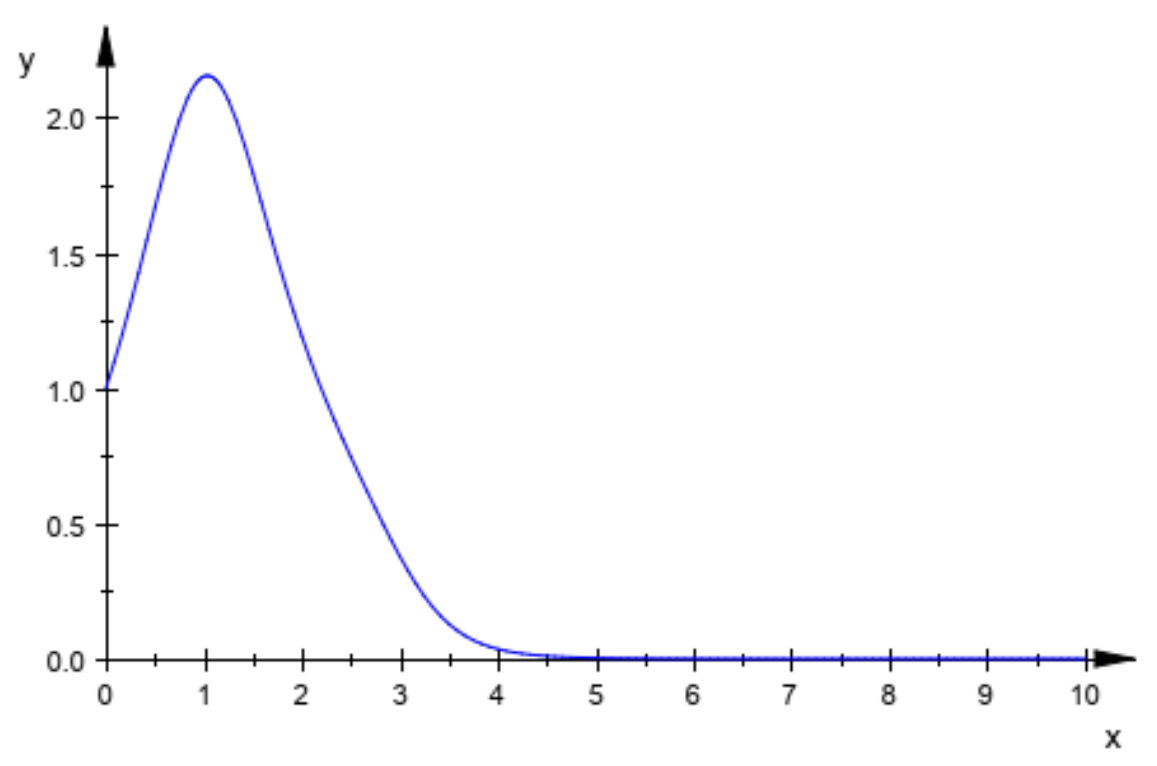
\includegraphics[width=0.5\textwidth]{./integral_approximation}
\end{figure}

\begin{enumerate}[label=(\alph*)]

\item Approximate the integral $I$ through uniform sampling at the five
points $x_k = 1, 3, 5, 7, 9$.

\[
\langle I \rangle = \sum_{k}  \frac{f(x_k)}{p(x_k)}
\]

Since there are five uniformly distributed points, the density for all of
them is $p = \frac{5}{10} = \frac{1}{2}$. What is the relative error of the
number you get?

\[
\begin{split}
\langle I \rangle
&= 2 \cdot \sum_k f(x_k) \\
&= 2 \cdot 2.5341479220696312 \\
&= 5.0682958441392625 \\
\end{split}
\]

The relative error is therefore:

\[
\frac{|5.0682958441392625 - 4.329268516|}{4.329268516}
= 0.1707\dots
\]

\item According to the idea of importance sampling, you concentrate the
evaluation of function values on the region where the values are largest i.e
. between 0 and 4 in our case. Sample the function at the points $x = 0.5, 1
.5, 2.5, 3.5$ as well as $x = 7$ and compute again the estimator $ \langle I
\rangle $ for the integral $I$. The density for the first four points (each
covering an interval of length 1) is $p = \frac{1}{1} = 1$ whereas the
density for $x = 7$ (which covers an integral of length 6) is $p =
\frac{1}{6}$.

\[
\begin{split}
\langle I \rangle
&= \sum_{k} p(x_k) \cdot f(x_k) \\
&= 4.338875262071001 \\
\end{split}
\]

The relative error from this is therefore:

\[
\frac{|4.338875262071001 - 4.329268516|}{4.329268516} \\
= 0.00221902292165451
\]


\end{enumerate}

\setcounter{enumi}{4}

\item Write down the directional form of the rendering equation. Briefly
explain each of the terms and the integration domain.

\[
L_0(\mathbf{x}, \stackrel{\to}{\omega}) = L_e(\mathbf{x},
\stackrel{\to}{\omega}) + \int_{H^2} f_r
(\mathbf{x}, \omega_i, \stackrel{\to}{\omega})
\cdot
L_i(\mathbf{x}, \omega_i)
\cdot
\cos\theta_i \text{d}\omega_i
\]

\begin{itemize}

\item $L_e(\mathbf{x},\stackrel{\to}{\omega})$ is the light emitted from the
point $\mathbf{x}$ in direction $\stackrel{\to}{\omega}$.

\item $\int_{H^2} \text{d}\omega_i$ integrates over all the angles in a
hemisphere $H$.

\item $L_0(\mathbf{x}, \stackrel{\to}{\omega})$ is the light emitting
emitted from $\mathbf{x}$ in the direction $\stackrel{\to}{\omega}$.

\item $f_r(\mathbf{x}, \omega_i, \stackrel{\to}{\omega})$ is the proportion
of the light incident from direction $\omega_i$ which is reflected in the
direction $\stackrel{\to}{\omega}$.

\item $L_i(\mathbf{x}, \omega_i)$ is the amount of light incident at the
point $\mathbf{x}$ from direction $\omega_i$.

\item $\theta_i$ is the angle between the normal and the incident ray.

\end{itemize}

\item Assume a scene containing only diffuse surfaces with diffuse
reflectance $\rho(x)$. The scene is surrounded by a single distant light
source with constant emission $\bar{L}$. Let $V(\mathbf{x},
\stackrel{\to}{\omega})$ be a function returning the visibility of the light
source from point $\mathbf{x}$ along direction $\stackrel{\to}{\omega}$.

Change/simplify the rendering equation you provided in (a) as much as
possible to estimate only direct illumination due to the light source.

\[
L_0(\mathbf{x}, \stackrel{\to}{\omega}) = \int_{H^2} \frac{\rho(x)\cdot
(\stackrel{\to}{\omega} - \stackrel{\to}{\omega}_i)
}{\pi} \cdot (\bar{L}\cdot V (\mathbf{x}, \stackrel{\to}{\omega}))
\cdot \cos \theta_i \text{d}\omega_i
\]

\item Recall the surface area form of the rendering equation:
\[
L(\mathbf{x}, \mathbf{z}) = L_e(\mathbf{x}, \mathbf{z}) + \int_A
f_r(\mathbf{x}, \mathbf{y}, \mathbf{z}) \cdot L(\mathbf{x}, \mathbf{y}) \cdot
G(\mathbf{x}, \mathbf{y}) \text{d}A(\mathbf{y})
\]

\begin{enumerate}

\item Provide the mathematical formulation of $G(\mathbf{x}, \mathbf{y})$
and explain its terms.

\[
G(\mathbf{x}, \mathbf{y}) = V(x, y)
\cdot \cos\theta_x \cdot \cos\theta_y
\cdot \frac{1}{|\mathbf{y} - \mathbf{x}|}^2
\]

{\color{blue}
$\mathbf{G}(x, y)$ is a geometry term. So $\mathbf{G}(x, y)$ contains the
angle, the visibility, the cosine between the normal and the cosine between
the angle and the normal at the light source.
}

\item Consider the following scene configuration. The rectangle $E$ on the
left is an area emitter with $L_e = 1$ and a black BSDF, ie.e. $f_r = 0$.
The coordinates of its corners are labeled. The ground plane is a
non-emissive surface with $f_r = \frac{1}{\pi}$. Provide pseudocode for a
Monte-Carlo estimator of $L$, given as input a point on the ground plane
$\mathbf{x}'$, a point on the camera $\mathbf{x}$ and the desired amount of
samples $N$. You can obtain numbers uniformly in $[0, 1)$ by calling
\texttt{RAND()}.

\begin{figure}[H]
\centering
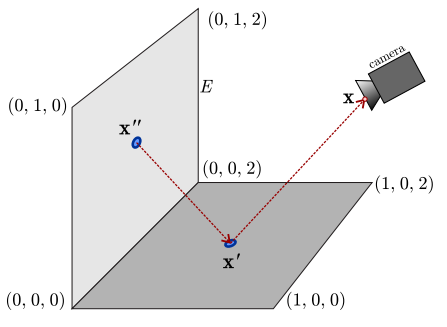
\includegraphics[width=0.5\textwidth]{./monte_carlo_exam_question}
\end{figure}

\begin{lstlisting}[escapeinside={'*}{*'}]
vector illumination(vector '*$\mathbf{x}$*', vector '*$\mathbf{x}'$*'){
	n = ...
	light = 0;
	for (int i = 0; i < n; i++{
		'*$\theta$*' = 2 * '*$\pi$*' * RAND();
		'*$\phi$*' = '*$\frac{\pi}{2}$*' * RAND();
		'*$\mathbf{y}$*' = '*$\begin{pmatrix} \sin\theta\cos\phi \\ \sin\theta\sin\phi \\ \cos\theta \\ \end{pmatrix}$*';
		if (intercepts_E('*$\mathbf{x} + \lambda\mathbf{y}$*')){
			light += '*$L_e$*' * '*$\cos\theta$*';
		}
	}
	return light / n * '*$\frac{\mathbf{x}}{|\mathbf{x}|}\cdot \begin{pmatrix} 0 \\ 1 \\ 0\\ \end{pmatrix}$*';
}
\end{lstlisting}

\end{enumerate}

\item Consider the following single-sample Monte Carlo estimator
$\langle F \rangle$ of an integral $F$ of an arbitrary non-negative integrand
$f(x)$ over an arbitrary domain $D$ with volume 1, driven by a random
variable $X\sim p(x)$.

\begin{align*}
F &= \int_D f(x)\text{d}x \approx \frac{f(X)}{p(X)} = \langle F \rangle, &
p(x) &= \frac{1}{2}\left( p_{\text{good}}(x) + p_{\text{bad}}(x) \right)
\end{align*}

The ``good'' probability density function $p_{\text{good}}(x)$ is
proportinoal to $f(x)$ and the ``bad'' probability density function
$p_{\text{bad}}$ is zero whenever $f(x)$ is non-zero.

Derive step-by-step the variance of the estimator $ \langle F \rangle $ as a
function of $F$.

\[
\begin{split}
p_{\text{good}}(x) &= c \cdot f(x) \Longrightarrow \\
\int^{\infty}_{-\infty} p_{\text{good}}(x) \text{d}x &=
\int^{\infty}_{-\infty} c \cdot f(x) \text{d}x \\
1 &= c \cdot \int_D f(x) \text{d}{x} \\
\frac{1}{c} &= \int_D f(x) \text{d}{x} \\
\end{split}
\]

Consider choosing a probability from the distribution $p$ as being a
binomial choice between $p_{\text{good}}$ and $p_{\text{bad}}$

\[
\begin{split}
E \left(\frac{f(X)}{p(X)}\right)
&= \sum p(x) \frac{\langle F(x) \rangle}{p(x)} \\
&= p_{\text{good}}(x) \frac{F(x)}{p_{\text{good}}(x)} \\
&= F(x) \\
\end{split}
\]

\[
\begin{split}
E\left( \langle F \rangle^2 \right)
&= \sum p(x) \langle F(x) \rangle^2 \\
&= p_{\text{good}}(x) \cdot \left(\frac{F(x)}{p_{\text{good}}(x)}\right)^2 \\
&= 2 \cdot F(x)
\end{split}
\]

\[
\begin{split}
\text{Var}(\langle F \rangle) &= E(\langle F \rangle^2) - E(\langle F
\rangle)^2 \\
&= 2 \cdot F^2 - F^2 \\
&= F^2 \\
\end{split}
\]

\item Consider a spotlight emitting radiant intensity $I = 20\frac{W}{sr}$
confined in a cone of directions with solid angle $\omega = 3 sr$. Compute
the total emitted radiant flux from this light.

\[
\Phi = \int^3_0 20\text{d}\omega = \left[20\right]^3_0 = 60W
\]

{\color{blue}
If you integrate over the square radians then you get the correct answer --
even though integrating over a square is nasty, it's like integrating over
the total area.
}

\end{enumerate}

\end{document}
